\chapter{Implementation}
\label{ch:Implementation}

In this chapter, we deduce the necessary equations to implement the reduction algorithm and present multiple optimizations.
We focus on summation, the reduction operator $\reduce$ will be floating-point addition.
While the recursive formula given in \Cref{eq:nodeReduceReduction} already defines a reduction algorithm, its implementation in imperative languages would heavily rely on the call stack to store intermediate results.
In practice, performing the calculations in opposite direction, from leaf nodes to the root, yields faster runtimes.

The binary representation of element indices has $\numLevels$ bits.
If we order them from most- to least-significant and interpret them as a series of decisions, where $0$ means \enquote{go up} and $1$ means \enquote{go right and up}, each index encodes a path from the tree root to the corresponding leaf node:

\begin{figure}[H]
\centering
\begin{tikzpicture}
\newcommand{\heightFactor}{0.7}
\newcommand{\treeN}{8}
\newcommand{\subtreeHeight}[2]{\directlua{tex.write(subtree_height(#1,#2))}}
\newcommand{\parentIdx}[1]{\directlua{tex.write(parent(#1))}}
\foreach \x in {0,...,\treeN} {
	\node [anchor=south] (idx\x{}) at (\x{},0) {\x};
	
	\draw (\x{},0)
		-- (\x{},-\heightFactor * \subtreeHeight{\x}{\treeN}-\heightFactor)
		-- (\parentIdx{\x},-\heightFactor * \subtreeHeight{\x}{\treeN}-\heightFactor);
}

% Highlighted path
\draw [very thick,red] (6,0) -- (6, -2 * \heightFactor) -- (4, -2 * \heightFactor) -- (4, -3*\heightFactor) -- (0, -3*\heightFactor) -- (0,-5*\heightFactor);
\node [red] at (0-0.3, -3.5*\heightFactor) {0};
\node [red] at (2, -2.5*\heightFactor) {1};
\node [red] at (5, -1.5*\heightFactor) {1};
\node [red] at (6-0.3, -0.5*\heightFactor) {0};

\draw [->,red] (-0.3,-\heightFactor * \subtreeHeight{0}{\treeN}-\heightFactor + 0.1) -- +(0,0.3);

\node at (10,-2) {$6_{10} = 0110_2$};
\end{tikzpicture}
\caption{Example path for index $6$ with $N = 9$}
\label{fig:indexTreePath}
\end{figure}

For any given $x$-coordinate $x > 0$, the \textbf{maximum $y$-coordinate} $\max_y(x)$ is equal to the number of trailing zeros of $x$, i.e.\ the zero-indexed position of the least-significant bit set in $x$.
We denote this expression as $\ffs (x) - 1$, where $\ffs$ is short for \enquote{find first bit set}.
The path representation explains why the equality holds: the least-significant bit set is the last time the $x$-coordinate changes along the path from the root, since all following bits are zero and encode the decision \enquote{go up}.

To find the $x$-coordinate of the \textbf{parent node} of an inner node $(x, \max_y(x))$, we replace the last (least-significant) \enquote{go right and up} decision with \enquote{go up}. 
Numerically, this is equivalent to cancelling the least-significant bit of $x$, which can be efficiently calculated using the bitwise AND-operation $'\BitAnd'$:

\begin{equation}
\label{eq:parent}
\textrm{parent} (x) := x \BitAnd (x - 1)
\end{equation}

Each \gls{pe} with rank $i$ (where $i \in [0, p - 1]$) stores $n_i$ consecutive elements.
The global index of the first element assigned to a \gls{pe} is the so-called start index, and it is equal to the prefix sum of the assigned number of elements:

\begin{align}
\textrm{startIndex} (0) &= 0 \\
\textrm{startIndex} (i) &= \sum_{j = 0}^{i - 1} n_i
\label{eq:startIndex}
\end{align}

This allows us to define the function rankFromIndex, which computes the index of the \gls{pe} that stores the given element:
\begin{equation}
\textrm{rankFromIndex} (x) = \max \{i \in [0, p - 1] \;|\; \textrm{startIndex} (i) \leq x \}
\end{equation}

For any given set $X$ of $x$-coordinates, we can use the rankFromIndex-function to determine the $x$-coordinates of outbound subtree roots, i.e. nodes whose parent node lies on a different \gls{pe}:

\newcommand{\rankIntersectingIndices}{I_{\textrm{\gls{pe}-intersecting}}}
\begin{equation}
\rankIntersectingIndices (X) = \{x \in X \;|\; \textrm{rankFromIndex} (x) \neq \textrm{rankFromIndex} (\textrm{parent} (x)) \}
\end{equation}

$largest\_subtree\_child\_index$ returns the largest $x$-coordinate of all child nodes of the given subtree root, which is equal to setting all trailing zeros of the given index to $1$.
This can be calculated using the bitwise OR-operation \enquote{|}:
\begin{equation}
\label{eq:LargestChildIndex}
largest\_subtree\_child\_index(index) = index \;|\; (index - 1)
\end{equation}

\begin{algorithm}
\caption{Summation procedure}\label{algo:SummationAlgo}
\KwData{\gls{pe}-rank $rank$, $n_{rank}$ summands with coordinates $(startIndex, 0)$ through $(startIndex + n_{rank} - 1,0)$}
\KwResult{Reduction result on the \gls{pe} with rank $0$}
\DontPrintSemicolon
\SetAlgoLined
$startIndex \gets startIndices (rank)$\;
$endIndex \gets startIndex + n_{\textrm{rank}}$\;
\uIf{$rank = 0$}{
	$outboundSubtreeRoots \gets \{0\}$\;
}
\Else{
	$outboundSubtreeRoots \gets \rankIntersectingIndices ([\textrm{startIndex}, \textrm{endIndex}))$\;
}
\For{$i \gets  outboundSubtreeRoots$}{
	\tcp{Reduce subtree level-by-level}
	\For{$y \gets [1, \max_y(x)]$}{
		\label{algo:SummationAlgoTopDownFor}
		$x \gets i$\;
		\While{$x \leq largest\_subtree\_child\_index(x)$}{\label{algo:SummationAlgoInnerLoop}
			$x_a \gets x$ \tcp*{$x$-coordinate of left child node}
			$x_b \gets x + 2^{y - 1}$ \tcp*{$x$-coordinate of right child node}
			$a \gets (x_a, y - 1)$ \tcp*{value of left child node}
			\uIf{$x_b \geq N$} {
				\tcp{No adjacent node, passthrough}
				$(x,y) \gets a$\;\label{algo:SummationAlgoPassthrough}
			}
			\uElseIf{$\textrm{rankFromIndex}(x_b) \neq rank$}{
				\tcp{\gls{pe}-intersecting node, fetch over \gls{mpi}}
				$b \gets \textrm{receive}\ (x_b, \max_y(x_b))$\;\label{algo:SummationAlgoRankIntersectingNode}
				$(x,y) \gets a + b$\;
			}
			\Else{
				$b \gets (x_b, y - 1)$\tcp*{value of right child node} \label{algo:SummationAlgoInnerNode}
				$(x,y) \gets a + b$\;
			}
			$x \gets x + 2^{y - 1}$\;
		}
	}
	\If{$rank \neq 0$}{
		$\textrm{send } (i, \max_y(i))$\;
	}
}
\end{algorithm}

\Cref{algo:SummationAlgo} shows the procedure that each \gls{pe} follows.
It consists of three nested loops.
The most outer loop iterates over all \gls{pe}-intersecting indices in ascending order; its body is responsible for the reduction of the subtree rooted at the corresponding \gls{pe}-intersecting node.
Because our reduction scheme is a left-leaning binary tree, nodes with lower indices occur earlier in the reduction equation, therefore processing \gls{pe}-intersecting indices in ascending order minimizes wait-times for other \glspl{pe}.


The inner loops in \Cref{algo:SummationAlgoTopDownFor} and \Cref{algo:SummationAlgoInnerLoop} implement the top-down scheme that reduces adjacent nodes level-by-level.
The distinctions made in Equations \eqref{eq:nodeReduceBaseCase}--\eqref{eq:nodeReduceReduction} give rise to a series of conditional expressions: \Cref{algo:SummationAlgoPassthrough} deals with inner nodes that have no adjacent node, \Cref{algo:SummationAlgoRankIntersectingNode} distinguishes between \gls{pe}-intersecting nodes and local inner nodes and \Cref{algo:SummationAlgoInnerNode} performs the local reduction of adjacent elements.

\section{Applied Optimizations}
\label{sec:AppliedOptimizations}

The implementation used in \Cref{ch:Experiments} follows \Cref{algo:SummationAlgo} with the following optimizations.
Message Buffering (\Cref{sec:MessageBuffering}) allows to reduce the number of messages sent across the network and therefore reduces the communication overhead.
The number of messages further decreases with a data distribution optimized for the reduction algorithm (\Cref{sec:DataDistribution}).
Vectorizing the additions (\Cref{sec:Vectorization}) yields the largest performance gain of all optimizations presented in this section.

\subsection{Message Buffering}
\label{sec:MessageBuffering}

\begin{figure}[H]
\centering
\begin{tikzpicture}
\newcommand{\heightFactor}{0.7}
\newcommand{\treeN}{5}
\newcommand{\subtreeHeight}[2]{\directlua{tex.write(subtree_height(#1,#2))}}
\newcommand{\parentIdx}[1]{\directlua{tex.write(parent(#1))}}
\foreach \x in {0,...,\treeN} {
	\node [anchor=south] (idx\x{}) at (\x{},0) {\x};
	
	\draw (\x{},0)
		-- (\x{},-\heightFactor * \subtreeHeight{\x}{\treeN}-\heightFactor)
		-- (\parentIdx{\x},-\heightFactor * \subtreeHeight{\x}{\treeN}-\heightFactor);
}

\draw [very thick, dashed, rounded corners, teal] (-0.5,0.5)  rectangle (2.4,-2.5);
\draw [very thick, dashed, rounded corners, olive]  (2.6, 0.5) rectangle (5.4,-2.5);
\node (PE0) at (1,1) {\gls{pe} 0};
\node (PE1) at (4,1) {\gls{pe} 1};

\fill[fill=red] (2,-1 * \heightFactor) circle [radius=2pt];
\fill[fill=red] (0,-3 * \heightFactor) circle [radius=2pt];

\end{tikzpicture}
\caption{Distributed tree with $N=6$ nodes and $p=2$ \glspl{pe}}
\label{fig:messageBufferingTree}
\end{figure}

Typically, low-index outbound subtree roots located on the same \gls{pe} have the same destination rank.
\Cref{fig:messageBufferingTree} is a minimal example for this observation: nodes $(3,0)$ and $(4,1)$ are outbound subtree roots that \gls{pe} 1 sends to \gls{pe} 0.
\gls{pe} 1 can avoid the additional message latency if it does not send $(3,0)$ directly, but stores it in a buffer instead.
Then, after finishing the computation of $(4,1)$, \gls{pe} 1 can send both results to \gls{pe} 0 in a single message.
Because \gls{pe} 0 calculates $(0,1)$ beforehand, the delayed transmission of $(3,0)$ does not impact the runtime negatively.

The current implementation utilizes a buffer with a maximum of $4$ elements per message.
After the summation routine has computed an outbound subtree root, it places the result in the outbound message buffer.
Flushing of the buffer occurs in either one of the following cases: \begin{itemize} 
\item The summation procedure inserts another outbound subtree root into the buffer which has a different target \gls{pe}.
\item The summation procedure begins work on an outbound subtree root whose subtree size is greater than $64$ summands. This guarantees an upper limit on the time a finished result spends inside the buffer.
\end{itemize}

The buffer utilization averages about $1.2$ summands per message, further tests have shown that relaxing above flushing criteria does not yield a runtime benefit, presumably because of the induced latency.

\subsection{Data Distribution}
\label{sec:DataDistribution}

If the user can arbitrarily assign elements to \glspl{pe}, multiple optimization techniques arise. To quantify them, we propose the following model:

\begin{equation}
\label{eq:distributionScore}
\textrm{Score} = t_{\textrm{MPI\_Send}} * n_{\textrm{\gls{pe}-intersecting nodes}} + \max \{ i \in [0, p - 1]\, |\, n_i * t_{\textrm{add}} \}
\end{equation}

$t_{\textrm{MPI\_Send}}$ is an estimate of the time needed to send a single element between two \glspl{pe}, $t_\textrm{add}$ estimates the time needed to add two floating-point values with double precision (64 bit).
On the shared-memory machine \textit{i10pc138}, these estimates were empirically measured to be $t_{\textrm{MPI\_Send}} \approx 281ns$ and $t_\textrm{add} \approx 4.15ns$.
While this model does not take any data dependencies between \glspl{pe} into account, it balances the performance gain achieved by parallelization (represented by a low maximum on the right side of \Cref{eq:distributionScore}) against the communication overhead caused by binary tree fragmentation. 

In this section we evaluate multiple approaches to the optimization of the data distribution with an example dataset with $N = 504\,850$ summands and $p = 256$ \glspl{pe}.

\subsubsection{Efficient message count determination}
To calculate the score in \Cref{eq:distributionScore}, an algorithm must efficiently determine the number of \gls{pe}-intersecting nodes.
A naive approach would be to check whether $rankFromIndex(parent(i)) \neq rankFromIndex(i)$ for each element $i \in \{0, \ldots, N-1\}$, requiring $O(N)$ time.

\Cref{algo:MessageCountSolver} represents a faster alternative requiring $O(p + \log_2 N)$ time.

\begin{algorithm}
\caption{Message count solver}\label{algo:MessageCountSolver}
\KwData{Distribution $n_i$, where $i \in \{0, \ldots, p - 1\}$}
\KwResult{Number of \gls{pe}-intersecting nodes}
\DontPrintSemicolon
\SetAlgoLined
$startIndices \gets \{\sum_{i=0}^j n_i \,\big|\, j \in [1, p-1] \}$\;
$messageCount \gets 0$\;
$i \gets 0$\; 
\While{$i + 1 < ranks$}{
	$startIndex = startIndices[i]$\;
	$endIndex = startIndices[i + 1]$\;
	$index = startIndex$\;
	\While{$index < endIndex$}{
		$messageCount \gets messageCount + 1$\;
		$index \ge´ts largest\_subtree\_child\_index(index) + 1$\;
	}
	$i \gets i + 1$\;
}
\KwRet{$messageCount$}
\end{algorithm}



\subsubsection{Even distribution}

\begin{table}
\centering
\begin{tabular}{l|l|l}
Distribution & Score & Message count \\
\hline
$n_i^\textrm{lower}$ & \SI{469.0}{\micro\second} & 1640 \\
$n_i^\textrm{upper}$ & \SI{401.9}{\micro\second} & 1401
\end{tabular}
\caption{Scores for the even data distribution ($N = 504\,850$, $p=256$)}
\label{table:EvenDistributionScores}
\end{table}
Distributing the data evenly, according to \Cref{eq:lowerDistribution} and \Cref{eq:upperDistribution}, ensures maximum parallelization of the computational effort, since the maximum difference in the workload of \glspl{pe} is $1$.
As shown in \Cref{table:EvenDistributionScores}, distributing the elements evenly yields a score of around $\SI{400}{\micro\second}$.
The advantages of the $n_i^\textrm{upper}$-distribution over the $n_i^\textrm{lower}$ distribution described in \Cref{sec:MessageCounts} express themselves in both a lower score and a lower message count.

\subsubsection{Round down to power of 2}
\label{sec:roundDownPower2Distribution}
The even distribution does not take the binary tree structure into account and may place \gls{pe}-boundaries at \enquote{inconvenient} places, producing numerous \gls{pe}-intersecting nodes.
By rounding down the number of assigned elements to the nearest power of $2$, we obtain start indices with a lot of trailing zeros, which is desirable since they produce larger \gls{pe}-local subtrees and reduce the number of \gls{pe}-intersecting nodes.
\Cref{eq:roundDownPower2Distribution} describes this approach formally.
The element count on the first $p - 1$ \glspl{pe} is a power of $2$.
By placing the remaining elements on the last \gls{pe}, we ensure that an uneven number of remaining elements does not reduce the trailing zeros of the start indices of the other \glspl{pe}.

\begin{equation}
\label{eq:roundDownPower2Distribution}
n_i^\textrm{power2} = \begin{cases}
2^{\lfloor \log_2 \frac{N}{p} \rfloor} & i < p - 1\\
N - \sum_{i=0}^{p-2} n_i^\textrm{power2} & i = p - 1
\end{cases}
\end{equation}

\begin{table}
\centering
\begin{tabular}{l|l|l}
Distribution & Score & Message count \\
\hline
$n_i^\textrm{power2}$ & \SI{1083.4}{\micro\second} & 256
\end{tabular}
\caption{Score of the $n_i^\textrm{power2}$ data distribution ($N = 504\,850$, $p=256$)}
\label{table:Power2DistributionScore}
\end{table}

The rounding decreases the amount of messages considerably (\Cref{table:Power2DistributionScore}).
With our test dataset, the message count is in the vicinity of the lower bound of $p - 1$, a $80\%$ reduction compared to the even distribution.
This comes at the cost of an imbalanced element distribution, the \gls{pe} with the highest rank, which stores the remaining elements, contains about half the elements.
The score function penalizes the inefficient parallelization with its the second term, causing the score to be $2.7\times$ higher compared to the even distribution.

\subsubsection{Optimized-Index Distribution}
As seen in \Cref{sec:roundDownPower2Distribution}, unbounded distribution optimization yields small message counts at the expense of computational imbalance.
In this section we will present a method to optimize the data distribution within certain bounds, to balance communication costs against computational costs.

Let $\textit{fairShare} := \tfrac{N}{p}$ be the approximate number of elements per \gls{pe} in an equivalent even distribution.
We want to optimize each $\textit{startIndex}(i)$ to produce the least amount of \gls{pe}-intersecting nodes while keeping the differences in the computational workload between \glspl{pe} small.
We express this requirement as follows:

\begin{equation}
\label{eq:optimizedIndexBounds}
\forall i \in \{1, \ldots, p - 1\}: \textit{startIndex}(i) - \textit{startIndex}'(i) \leq \alpha * \textrm{fairShare}
\end{equation}
where $\textit{startIndex}'(i)$ is the optimized start index and $\alpha$ is the maximum deviation relative to the even distribution.
In \Cref{algo:optimizeIndex}, we iteratively improve our start index by applying the \textit{parent}-function (\Cref{eq:parent}) until the proposed index violates \Cref{eq:optimizedIndexBounds}.
We obtain the complete data distribution $n_i^\textrm{optimized}$ by executing \Cref{algo:optimizeIndex} on each start index of the $n_i^\textrm{upper}$-distribution.

\begin{algorithm}
\caption{Index optimization procedure}\label{algo:optimizeIndex}
\DontPrintSemicolon
\SetAlgoLined
\KwData{\gls{pe}-rank $i$, start index $j$, maximum deviation parameter $\alpha$}
\KwResult{Optimized start index for the \gls{pe} with rank $i$}

$currentIndex = j$\;
$proposedIndex = currentIndex$\;

\While{$\textrm{initialIndex} - \textrm{proposedIndex} \leq \alpha * \tfrac{N}{p}$} {
	$currentIndex = proposedIndex$\;
	$proposedIndex = parent(initialIndex)$\;
}
\Return $currentIndex$\;
\end{algorithm}


\begin{table}
\centering
\begin{tabular}{l|l|l}
Distribution & Score & Message count \\
\hline
$n_i^\textrm{optimized}$ & \SI{184.5}{\micro\second} & 621
\end{tabular}
\caption{Score of the $n_i^\textrm{optimized}$ data distribution ($N = 504\,850$, $p=256$)}
\label{table:Power2DistributionScore}
\end{table}

\Cref{fig:distribution_runtimes} shows a histogram of the summation duration measured over $4\,000$ repetitions for our test dataset with a maximum deviation of $\alpha = 0.2$.
The runtime benefit of an optimized data distribution is visible, with optimized distribution the algorithm calculates results about $\SI{4}{\micro\second}$ faster than with  an even distribution.

\begin{figure}
\centering
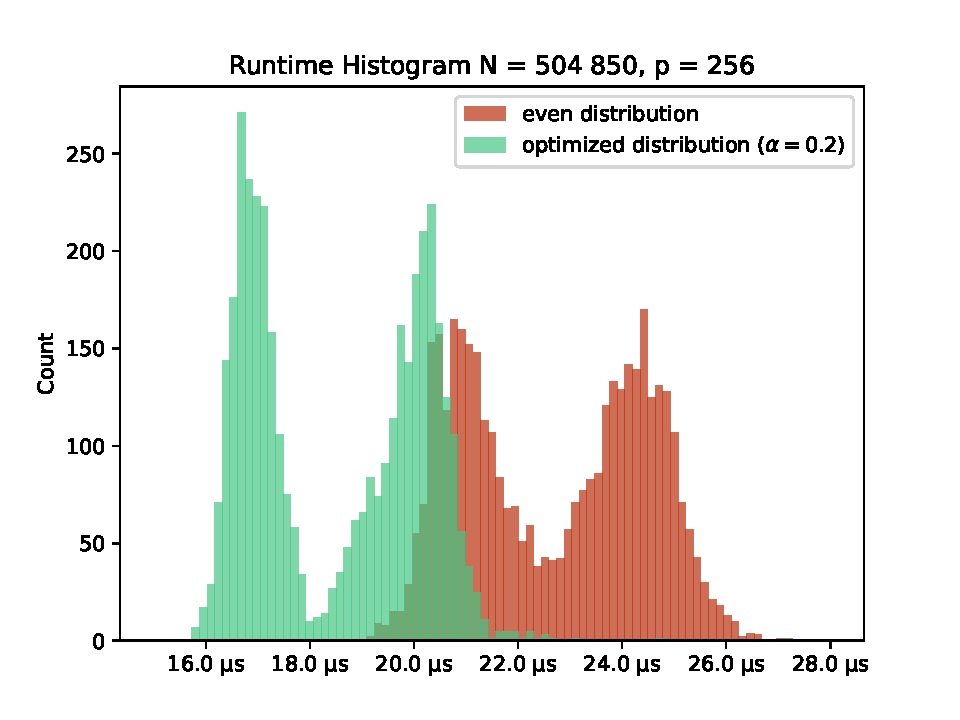
\includegraphics[scale=0.75]{figures/distribution_experiment}
\caption{Runtime comparison of even vs.\ optimized data distribution}
\label{fig:distribution_runtimes}
\end{figure}


\subsection{Index-lookup Hashmap}
\label{sec:IndexLookupHashmap}

\begin{figure}
\centering
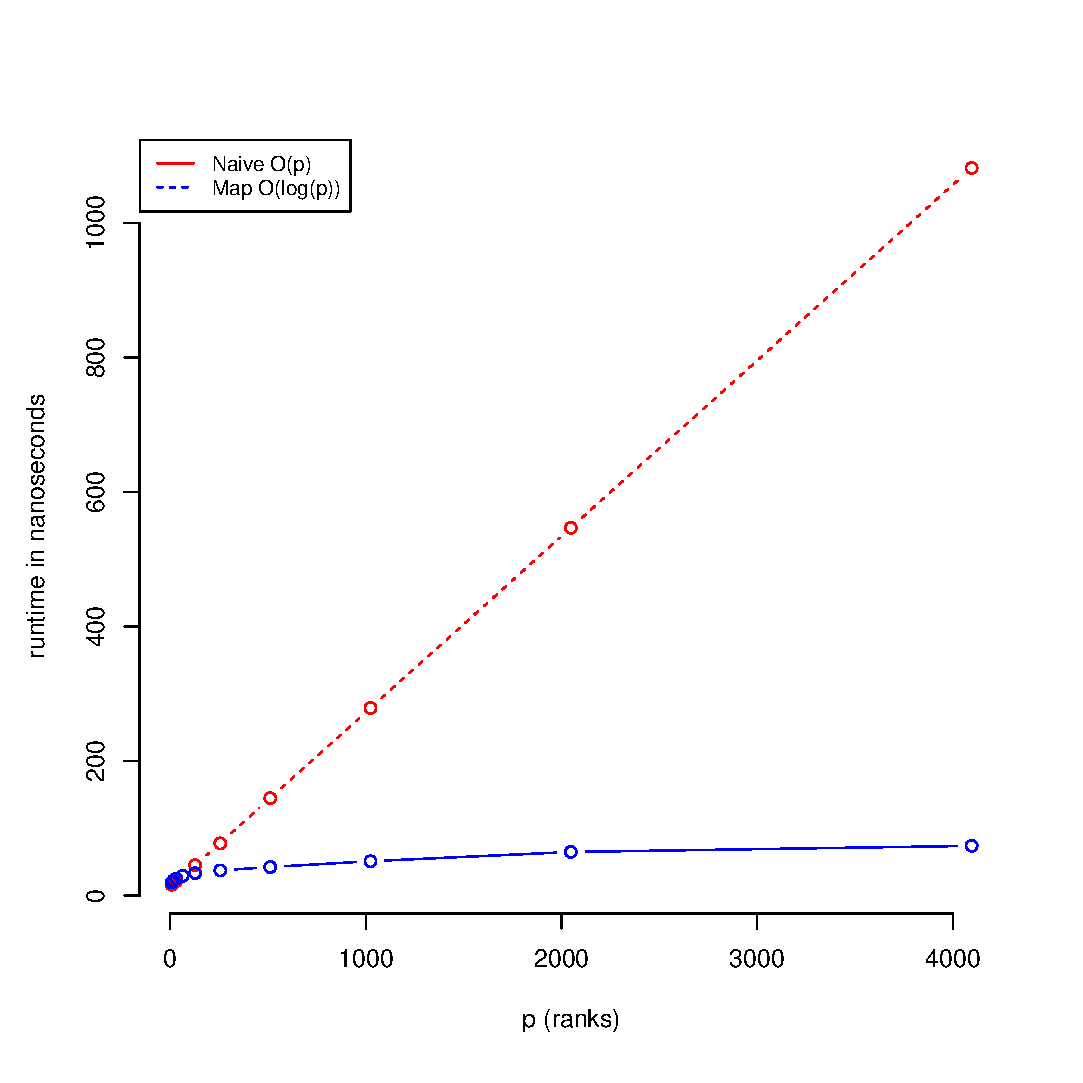
\includegraphics[scale=0.55]{figures/microbenchmark_rank_from_index.eps}
\caption{Microbenchmark comparison of unoptimized and optimized $rankFromIndex$ function}
\label{fig:microbenchmarkRankFromIndex}

\end{figure}

\Cref{algo:SummationAlgo} uses the $rankFromIndex$ function to lookup the \gls{pe}-rank for a given element index.
This function maps the binary tree structure to the underlying computing topology and its execution speed is performance-critical due to its position inside a frequently executed loop.

The initial implementation used a loop to find the first entry in the \textit{startIndices} array which numerically exceeds the input index.
The runtime of this algorithm is $O(p)$.
Microbenchmarks revealed the linearly increasing runtime and the need for optimization (see \Cref{fig:microbenchmarkRankFromIndex}).
The currently implemented version uses a hash map to scan for the start index, which yields a runtime in $O(\log(p))$.

\subsection{Vectorization}
\label{sec:Vectorization}

\begin{figure}
\begin{tikzpicture}[
block/.style={draw,minimum width=1.6cm, text centered,minimum height=0.8cm,font=\small}]

\node[block,left=0.8cm of {0,0}](d){$D$};
\node[block,left=0cm of d](c){$C$};
\node[block,left=0cm of c](b){$B$};
\node[block,left=0cm of b](a){$A$};




\node[block,right=0.8cm of {0,0}](e){$E$};
\node[block,right=0cm of e](f){$F$};
\node[block,right=0cm of f](g){$G$};
\node[block,right=0cm of g](h){$H$};



\node[block,below=2cm of {-2.4,0}](ab){$A+B$};
\node[block,right=0cm of ab](ef){$E+F$};
\node[block,right=0cm of ef](cd){$C+D$};
\node[block,right=0cm of cd](gh){$G+H$};

\node[below=0.8cm of {0,0}](op1) {$\_mm256\_hadd\_pd$};
\path[->,very thick] (c) edge (-1.6,-2);
\path[->,very thick] (f) edge (1.6,-2);

\node[block,below=4cm of c](ab2){$A+B$};
\node[block,right=0cm of ab2](ef2){$E+F$};
\node[block,below=4cm of e](cd2){$C+D$};
\node[block,right=0cm of cd2](gh2){$G+H$};
\path[->,very thick] (-1.6,-2.8) edge (-2.4,-4.4);
\path[->,very thick] (1.6,-2.8) edge (2.4,-4.4);
\node[left=0.6cm of {-2.0,-3.6}] (op2) {$\_mm256\_extractf128\_pd$};
\node[right=0.6cm of {2.0,-3.6}] (op3) {$\_mm256\_castpd256\_pd128$};

\node[block,left=0cm of {0,-7}](abcd){$(A+B)+(C+D)$};
\node[block,right=0cm of abcd](efgh){$(E+F)+(G+H)$};
\path[->,very thick] (-2.4,-5.2) edge (-2,-6.6);
\path[->,very thick] (2.4,-5.2) edge (2,-6.6);
\node[above=0.4cm of {0,-6.6}](op4) {$\_mm\_add\_pd$};

\node[block,left=0cm of {0,-9}](abcdefgh){$((A+B)+(C+D))+((E+F)+(G+H))$};
\node[block,right=0cm of abcdefgh](abcdefgh2){$((A+B)+(C+D))+((E+F)+(G+H))$};
\path[->,very thick] (0,-7.4) edge (0,-8.6);
\node[right=0.4cm of {0,-8}](op5) {$\_mm\_hadd\_pd$};

\end{tikzpicture}
\caption{Register content during AVX-2 subtree summation}
\label{fig:avxSchema}
\end{figure}

\begin{figure}
\centering
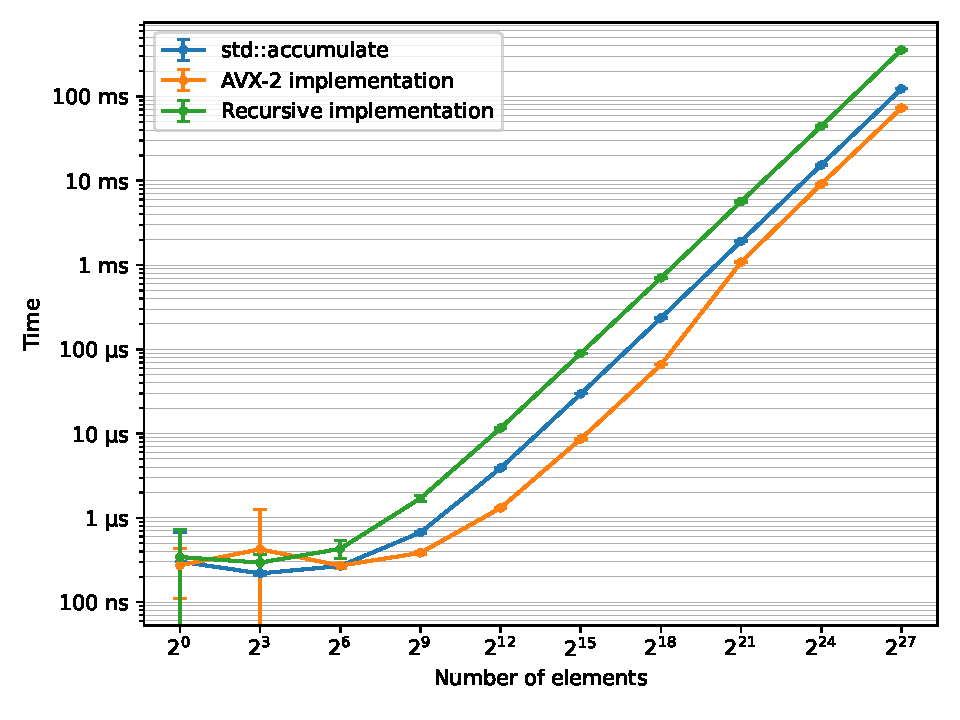
\includegraphics[scale=0.75]{figures/benchmarkVectorization}
\caption{Microbenchmark comparing sequential summation to AVX-2 binary tree reduction for $p=1$}
\label{fig:benchmarkVectorization}
\end{figure}

The theoretical per-node peak of \gls{flops} increases dramatically under the utilization of \gls{simd} capabilities~\cite{dolbeau_theoretical_2018}.
While modern compilers try to automatically vectorize existing code, optimization by hand can yield better results.

Compared to the simple left-to-right reduction presented in \Cref{sec:SequentialLeftToRightReduction}, a reduction tree lends itself better to parallelization, since an algorithm can reduce subtrees independently.
The implementation at hand uses x86 \gls{avx}, specifically AVX-2.
AVX-2 registers are $256$ bits wide and can therefore store four double precision floating-point numbers.
\Cref{algo:AVXTreeAccumulation} uses two registers to accumulate a subtree of eight elements at once.
Because AVX-2 instructions manipulate data within 128-bit lanes, it is necessary to extract the upper 128-bit after the first horizontal add in order to follow the correct summation order.
\Cref{fig:avxSchema} displays the register contents over time.
\begin{algorithm}
\caption{8-tree summation with AVX-2 instructions}
\label{algo:AVXTreeAccumulation}
\DontPrintSemicolon
\SetAlgoLined
\KwData{Buffer \textit{buffer} with at least $8$ entries at offset $i$}
\KwResult{Subtree sum of $8$ elements}

$a \gets mm256\_load\_pd(buffer[i])$\;
$b \gets mm256\_load\_pd(buffer[i + 4])$\;
$level1Sum \gets mm256\_hadd\_pd(a,b)$\;

$c \gets mm256\_extractf128\_pd(level1Sum 1)$\;
$d \gets mm256\_castpd256\_pd128(level1Sum)$\;
$level2Sum \gets mm\_add\_pd(c, d)$\;

$level3Sum \gets mm\_hadd\_pd(level2Sum, level2Sum)$\;

\Return $mm\_cvtsd\_f64(level3Sum)$\;
\end{algorithm}

The implementation at hand uses \Cref{algo:AVXTreeAccumulation} as a subroutine inside \Cref{algo:SummationAlgo} to advance the iterative reduction three levels per iteration.
If the remaining number of elements in the current iteration is not divisible by eight, the algorithm processes the remaining elements using non-vectorized instructions.
\Cref{fig:benchmarkVectorization} compares the runtime of the \texttt{std::accumulate} routine from the C++ standard library against the implementation at hand.
Since only one \gls{pe} executes this microbenchmark, no communication takes place and all runtime costs are purely computational.
For smaller workloads ($N < 64$), the overhead introduced by the vectorization is larger than the performance gains, but for larger workloads the AVX-2 implementation outperforms \texttt{std::accumulate}.
